% !Mode:: "TeX:UTF-8"

\chapter{基于局部分步式矩阵分解的可解释性地点推荐系统}
\label{chapter:main3}

推荐系统旨在积极准确地为用户提供有趣的信息或服务。一直以来,推荐系统都是企业的研究重点,良好的推荐系统可以为企业带来更多的收入。如今,推荐系统的准确性越来越高,其潜藏的可解释性渐渐得到了研究人员的关注。本章将改进最普适的基于矩阵分解的协同过滤算法并提出一种具有良好解释性的算法。

\section{问题描述}
在所有推荐方法中,基于矩阵近似(MA)的协同过滤(CF)方法被证明非常简洁和有效。最初,在只有用户-商品交互评分数据可用的时候,研究人员将用户和商品都看成独立个体并简单地将评分矩阵分解为两个低秩矩阵\citeup{paterek2007improving,weightedSVD,mnih2008probabilistic,rennie2005fast,salakhutdinov2008bayesian}。以这种方式,用户的偏好和商品的属性便可以体现在这低秩的潜在向量中。当通过取用户向量和商品向量的内积时候,缺失的评分值便可以被预测出来。

这种基于矩阵分解架构的推荐系统效果是喜人的,然而目前主流方法都忽略了一项最重要的任务:探索推荐结果背后的原因。具体来说,无论特征工程的精细程度如何,这些方法的核心都是不具备直观意义的隐向量,没有解释意义。这使得使推荐系统像黑盒一样工作。



\begin{figure}[t!]
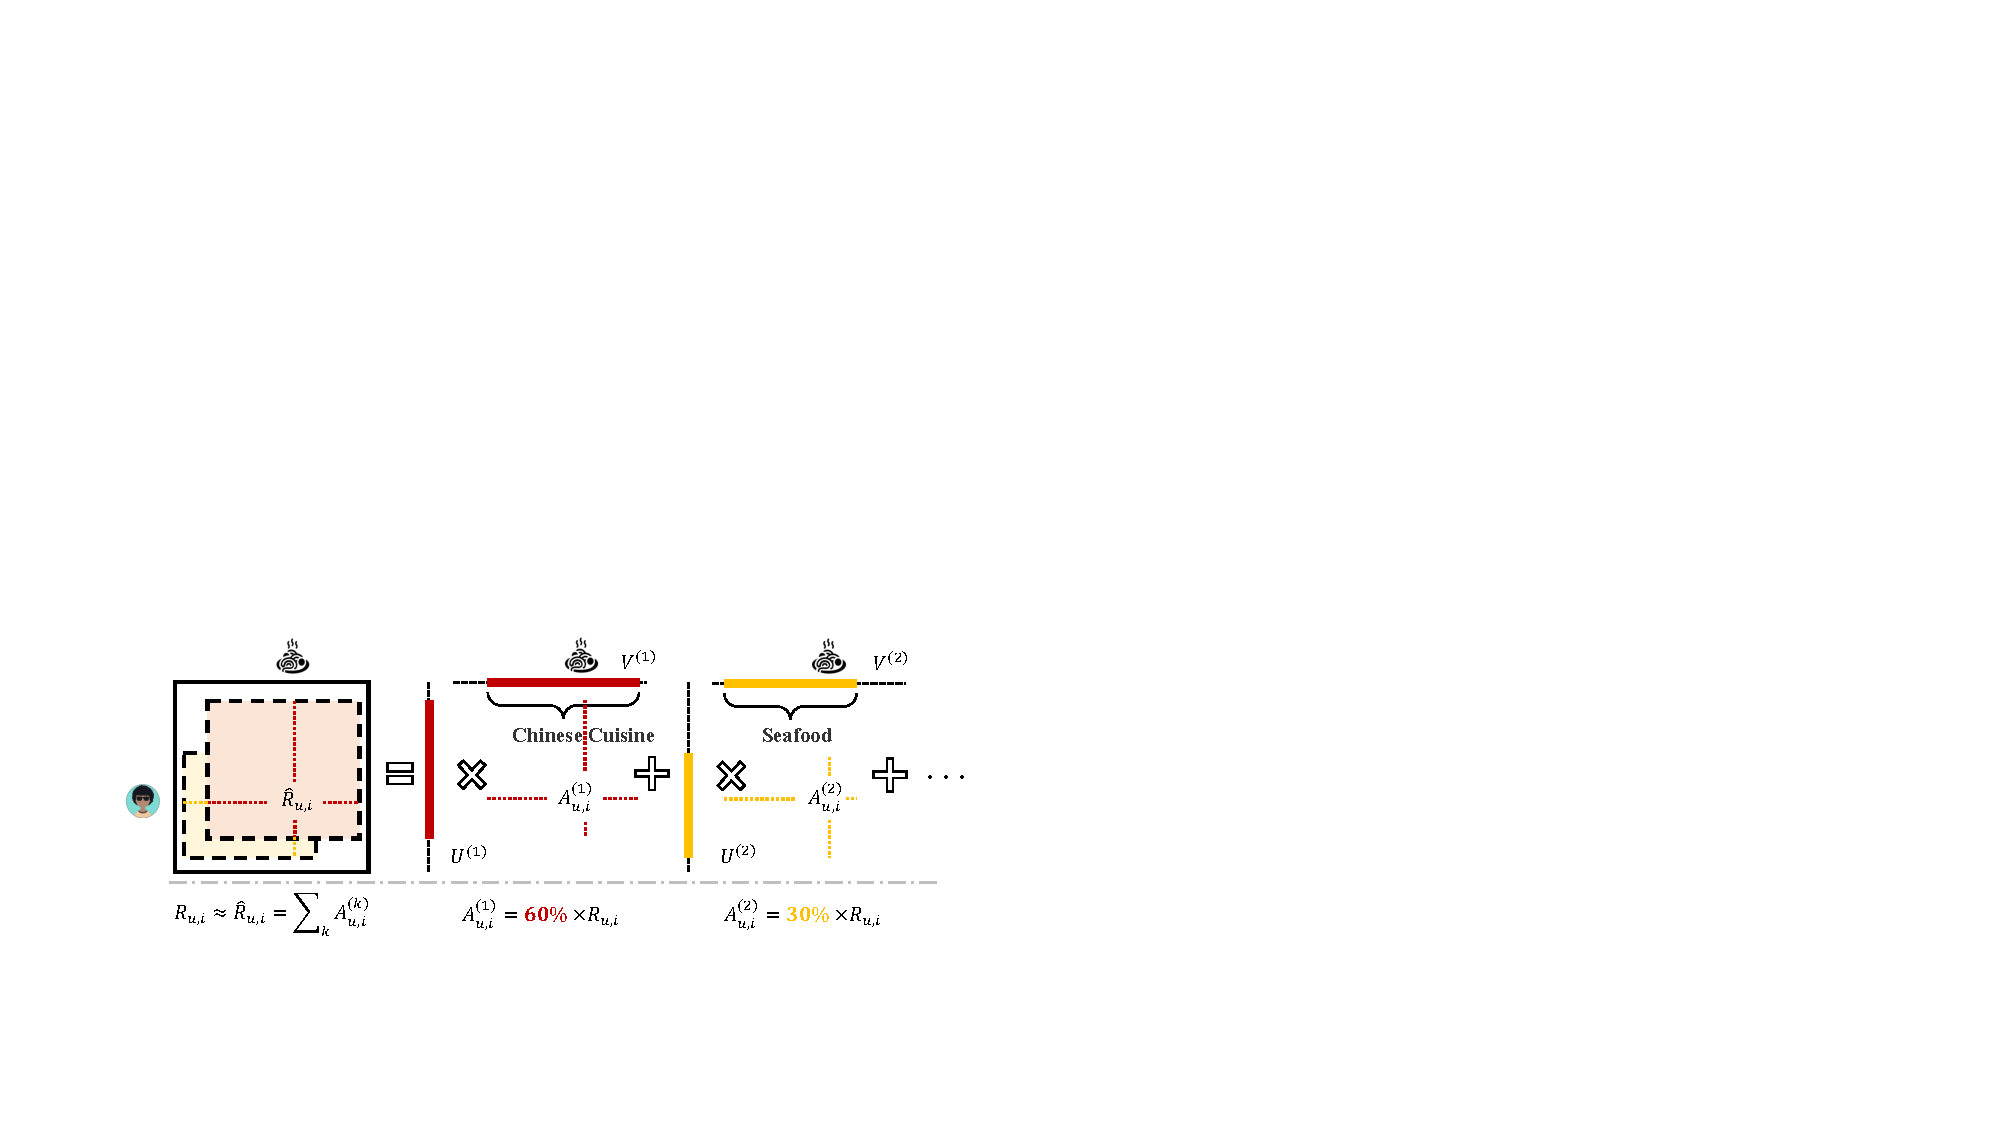
\includegraphics[width=\textwidth]{pics/explain.pdf}
\caption{基于矩阵分解的可解释推荐系统示意图。$U^{(1)},U^{(2)},V^{(1)}$ 和$V^{(2)}$ 是分解出来的向量。虚线部分代表0。} 
\label{explain}
\end{figure}

实际上,正如Ribeiro等人\citeup{ribeiro2016should}提到的:如果用户不信任一个模型,他们就不会放心地使用它。相反,如果模型在做出推荐的时候给出解释,即使结果可能不是最优的,用户也可以接受。此外,了解模型背后的原因可以帮助研究人员发现问题并升级他们的方法。在推荐系统中考虑下面的例子:当向用户推荐一个辛辣的中国海鲜面条时,系统不会明确地指出“其他用户也喜欢它”,而是说“这个推荐结果是根据你的口味量身定制的,其中包含$ 60\%$的中国菜因素,$ 30\%$的海鲜因素以及$10\%$的其他因素。尝一尝?”如果这个解释引起了用户的兴趣,那么它可以赢得用户的信任。为此,我们提出了一个局部分步秩一矩阵分解模型(BLOMA)模型,图\ref{explain}说明了BLOMA的基本逻辑,与传统的基于矩阵分解的协同过滤方法相比其有三个主要差异:1)评级矩阵在部分用户和商品上进行局部分解,2)仅对前一步骤获得的残差矩阵进行分解,而不是原矩阵,以及3)每个分解是秩一分解,其仅产生一个用户矢量和一个商品矢量。这三个变化将共同使得分解出的隐向量的主题更加明显,例如,向量 $ V ^ {(1)} $和$ V ^ {(2)}$中的大多数值分别代表中国菜和海鲜。在本文中,我们将描述BLOMA的细节并讨论其性能。% 此处先介绍传统矩阵分解模型以及其扩展。





\section{具有解释性的局部分步矩阵分解模型}
\label{main}

\subsection{矩阵分解模型及其扩展}
基于矩阵分解的协同过滤模型的基本假设是将用户和商品用等长的隐向量表示为:\gls{U}$\in \mathbb{R}^{m\times r}$ and \gls{V} $\in \mathbb{R}^{r \times n}$,并使它们的乘积尽量接近\gls{R} $\in \mathbb{R}^{m\times n}$,使得$R \approx UV$。其中$m$是用户数目,$n$是商品数目,$r$是隐空间的秩,满足$r \ll \min(m,n)$。为了防止过拟合,一般会在$U$和$V$上加正则项,整个目标损失为:
\begin{equation}
\label{base}
\argmin_{U,V} \sum_{(u,i)\in \Omega} (R_{ui}-U_u V_i)^2 + \frac{\lambda_1}{2}\|U\|_F^2 + \frac{\lambda_2}{2}\|V\|_F^2,
\end{equation}
其中 $\lambda_1,\lambda_2 > 0$是控制正则项强弱的系数。$\|\cdot\|_F$表示二范数。$U_u \in \mathbb{R}^{1\times r}$是表示用户$u$的行向量,$V_i \in \mathbb{R}^{r\times1}$是表示商品$i$的列向量。 $\Omega_{ui}$为指示函数,当取值为$1$时代表用户$u$与商品$i$有过交互。

在协同过滤的场景下,该模型过于笼统,因为它一次考虑所有用户和商品,因此无法正确解释特定用户或商品独特的特征。这就是为什么引进基于局部矩阵近似(Local Matrix Approximation, LMA)的方法的原因。

\smallsection{局部分解模型}
通常情况下,用户仅对一部分商品感兴趣,且每个商品也吸引不到所有用户。因此,评分数据中存在很多子簇。为了挖掘这些子簇结构,很多工作\citeup{lee2013local,zhang2014understanding,chen2015wemarec,li2017mixture,zhao2017collaborative,zhang2017local}提出了各自的解决方案。如果全局的矩阵分解只能表达一种“共同利益”,那么LMA则可以发现特定用户或商品拥有的“独特兴趣”。损失函数可以写成如下:
\begin{equation}
\label{localMF}
\argmin_{U^{(1\cdots K)},V^{(1\cdots K)}} \sum_{(u,i)\in \Omega} (R_{ui}- \sum_{k=1}^K{U^{(k)}_uV^{(k)}_i})^2 + \frac{\lambda_1}{2}\sum_{k=1}^K\|{U^{(k)}}\|_F^2 + \frac{\lambda_2}{2}\sum_{k=1}^K\|{V^{(k)}}\|_F^2,
\end{equation}
其与式(\ref{base})的区别是原用户和商品的隐藏因子矩阵$U,V$将被替代为一系列的子矩阵$U^{(1\cdots K)},V^{(1\cdots K)}$,其中$K$是子矩阵的个数。由于减小了每次分解的用户数和商品数,算法效率也会大大提升。




\begin{figure}[t!]
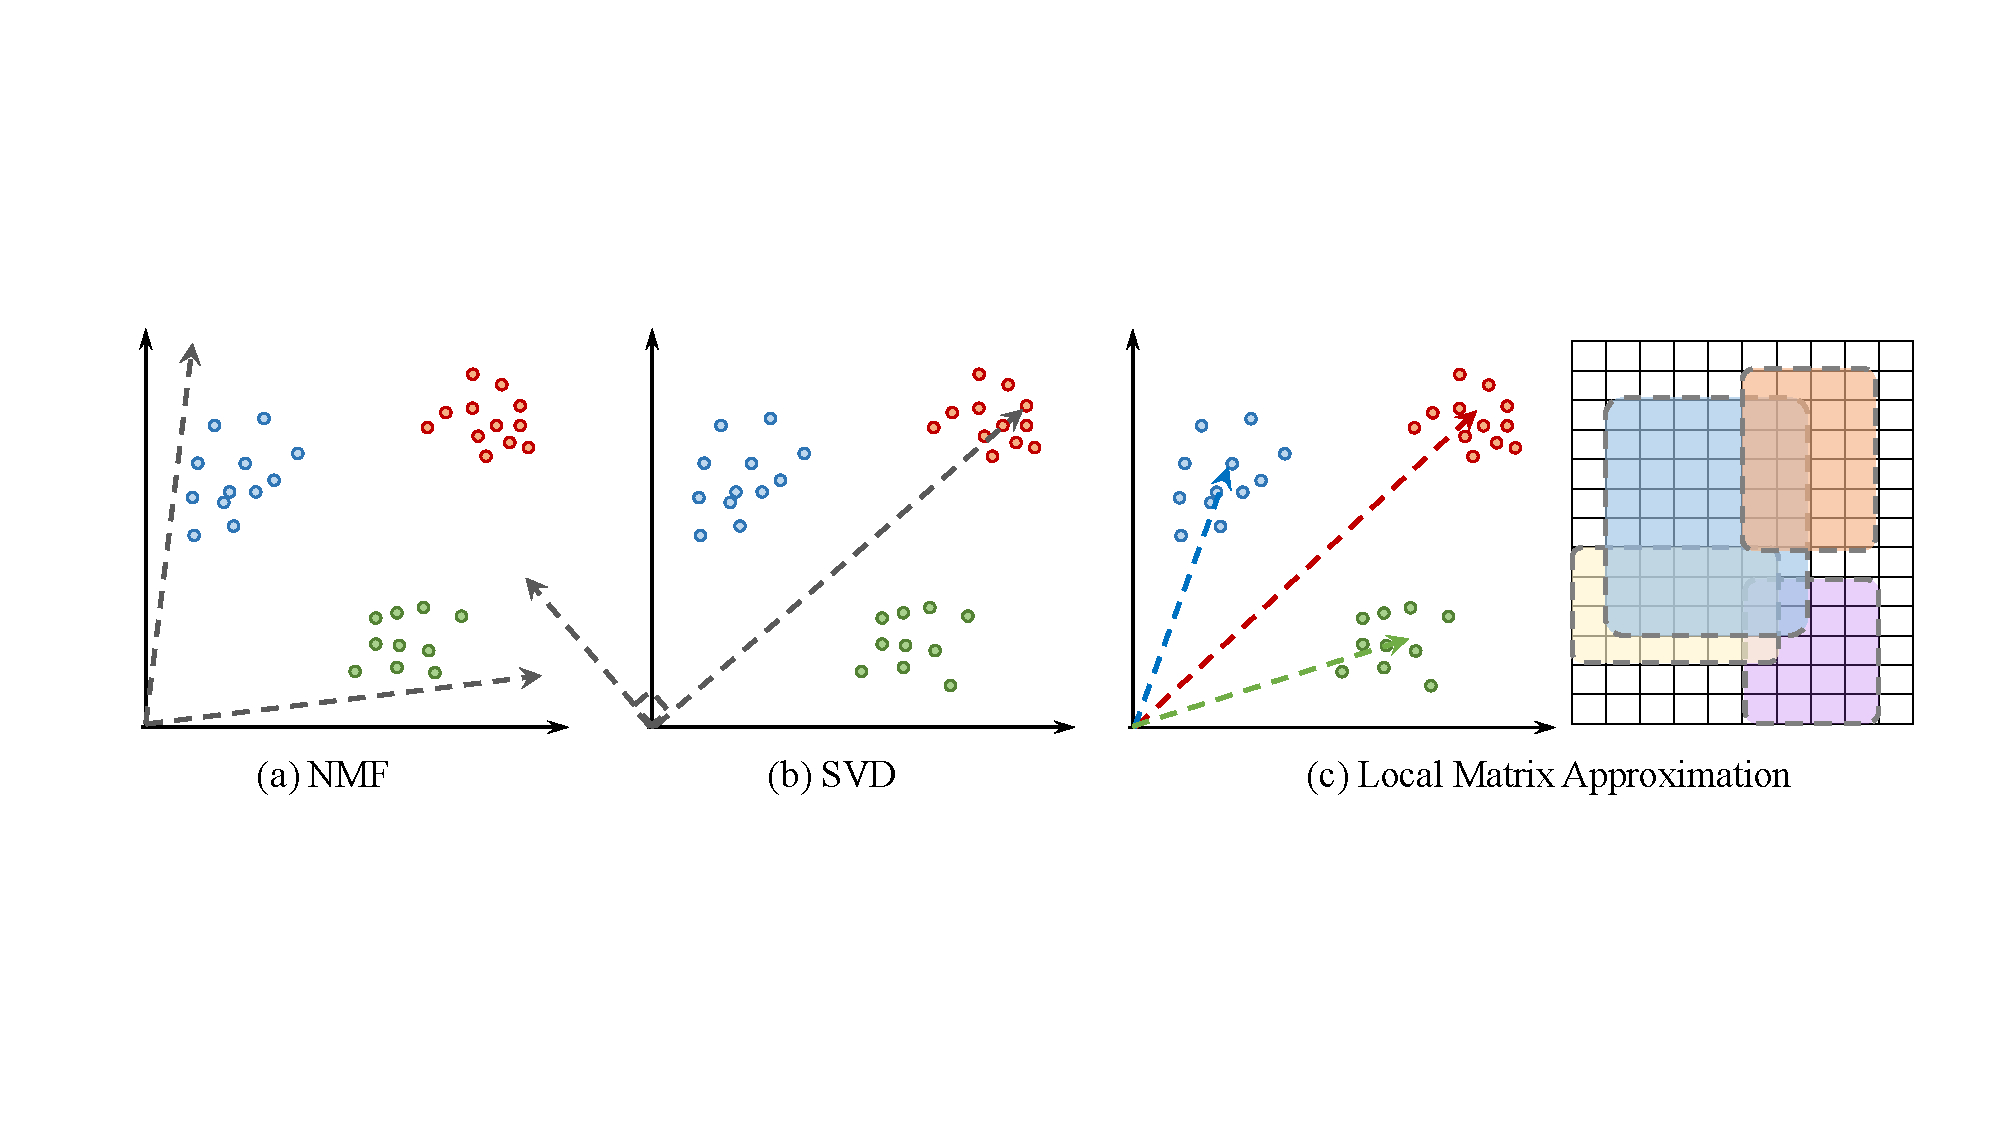
\includegraphics[width=145mm]{pics/compare.pdf}
\caption{三种不同模型的工作原理。} \label{compare}
\end{figure}
我们在图\ref{compare}中说明了非负矩阵分解(NMF),奇异值分解(SVD)和LMA工作原理。假设在潜在空间中存在三个簇,其代表三种主题,例如为中餐,印度餐馆和墨西哥餐馆。x轴和y轴可以表示辣的程度以及与市中心的距离等一些高级特征。从图中可以看到NMF和SVD可以准确地近似矩阵,但是他们不能直接发现商品中的三个主题,这是因为他们只追求潜在因素的组合应该接近训练集中的评分值。而LMA模型首先就探索了用户和商品之间的相关性,因此可以轻松区分每一个主题,使得发现的隐向量更直观和可解释。


然而在LMA模型中还是有两个问题:
\begin{enumerate}
\vspace{1.5mm}
\item \textbf{如何选择隐因子维度$K$,即式(\ref{localMF})中子矩阵的数量?} 这个问题类似于如何选取$k$-means算法中的$K$一样,是模糊和启发式的。如Zhao等人\citeup{zhao2017collaborative}所述,$K$的增大将使得误差减小,但极端情况下每个子矩阵只包含一个用户和商品的交互,这样模型就没意义了。此外由于最终预测结果是由一系列局部矩阵组合而成,因此性能也将由它们决定。但是这些本地子系统是独立工作的,在组合它们时候并没有周全的集合策略。这促使我们使用Freund等人\citeup{freund1999short}的工作来提出BLOMA模型以便解决这个问题。

\vspace{1.5mm}
\item \textbf{如何找寻子矩阵包含的用户集与商品集?}这个问题有很多策略,Shao等人 \citeup{shao2017synchronization}用了一种双边聚类的方式自动找寻;Zhang等人\citeup{zhang2013improve}提出了一种社团挖掘的方式来找寻关系紧密的用户和商品。Mackey等人\citeup{mackey2011divide}和Lee\citeup{lee2013local}等人用了分治法的思想来解决这个问题。Zhao等人\citeup{zhao2017collaborative}利用了社交信息,用朋友关系来找寻用户社区。然而这些方法都是独立的考虑各种信息,没有有机结合起来,因此在BLOMA模型中我们综合考虑了评分矩阵以及社交信息和商品的属性信息,使得找寻的用户社团和商品类更加全面。
\end{enumerate}

\subsection{融入集成学习机制的局部矩阵分解}
考虑上面列出的挑战,我们通过借用从集合学习中逐步推进的方式来解决\citeup{freund1999short}。思路是分步地对矩阵进行分解,在第$k$阶段获得第$k$个局部的因子,这和上面LMA模型不同的地方在于LMA是同时获得$K$个隐因子的。而我们选择迭代式分解原评分矩阵$R$。更具体地说,在第$k$阶段,我们仅仅拟合第$(k-1)$阶段的评分矩阵残差\gls{R_k},这个残差矩阵可写为:
\begin{equation}
\label{residue}
R^{(k)} = 
\begin{cases}
R& \text{if } k=1,\\
R^{(k-1)}-U^{(k-1)}V^{(k-1)}& \text{otherwise}.
\end{cases}
\end{equation}
它也可以展开为:
\begin{equation}
\label{unfold}
R^{(k)} = \bigg(\Big(\big(R-U^{(1)}V^{(1)}\big) - U^{(2)}V^{(2)} \Big)-\cdots-U^{(k-1)}V^{(k-1)}\bigg),
\end{equation}
在这一个阶段,模型仅仅集中拟合残差矩阵$R^{(k)} \approx U^{(k)}V^{(k)}$而不管之前的步骤。本文中我们用了秩一矩阵来作为分解基石,即让$U^{(k)}$和$V^{(k)}$成为一个向量而非矩阵,这样的好处有两个(1)仅仅有一个维度,不需要考虑多维度之间的耦合,于是每个阶段发掘的商品主题可以更加明确,这有助于推荐系统的可解释性。
(2)计算复杂度更低。 虽然存在近似误差,但可以在下一阶段进继续拟合消除这个误差。

注意国际上也有其他工作\citeup{biggs2008nonnegative,ensnmf,li2018multi}的思想类似于我们的BLOMA模型,都采用了集成学习这种分步学习的方式,但Suh等人\citeup{ensnmf}和Biggs等人\citeup{biggs2008nonnegative}是将这种技术应用到了NMF中,这并不适合我们的局部矩阵分解的场景。原因是当从原始矩阵中减去局部近似时,残差矩阵将不能保证非负性了。在他们的工作中,他们只是强制所有负值为零,这将在每个阶段中引入误差。Lee等人在没有非负约束的情况下将这种集成思想应用于矩阵分解,然而,他们只是以全局方式运行他们的模型而不仔细考虑矩阵的局部分解。

\subsection{子矩阵的构建}
先前的工作要么使用评分数据,要么使用社交网络进行抽样,他们都没有将这些异构来源组合在一起。 本文提出了一种同时利用评分数据和其他附加信息的子矩阵构造方法。主要分为两个步骤,核心用户和项目选择以及邻居搜索。这里定义了两种邻居,即根据评分矩阵选取的邻居和根据附加信息选取的邻居。

\smallsection{核心用户和核心商品的选取}
BLOMA模型的核心思想就是估计上一阶段没有拟合好的残差矩阵\gls{R_k},这最容易想到的思路就是找寻$R^{(k)}$中绝对值较大的部分来进行拟合。具体来说,选取一个在残差矩阵中剩有很大未被解释部分的核心用户$u \in \mathcal{U}$和一个核心商品$i \in \mathcal{I}$,然后找寻它们的邻居来构造局部矩阵分解的子矩阵。其中核心用户$u$和核心商品$i$中没被解释的部分被定义为残差矩阵中行$R_{u,\cdot}^{(k)}$和列$R_{\cdot,i}^{(k)}$的和。因此本文以$\sum_i|(R_{u,i}^{(k)})|/\sum_{u,i}|(R_{u,i}^{(k)})|$的概率来采样出一个核心用户$u$,采样核心商品$i$的方法也一样,不再赘述。

\smallsection{评分矩阵中的邻居选取}
考虑到我们想要找到具有相同特征的用户群体和商品类这一动机,我们选择一组与核心用户$ u $和核心商品$ i $分别具有高相似度的用户和商品。这一相似度我们用反余弦距离来判断,在Lee等人\citeup{lee2013local}的工作中提供了相关依据。用户$ u_1 $和$ u_2 $间的反余弦值定义为
\begin{equation}
\label{arc-cosine}
d(u_1,u_2) = \arccos(\frac{R_{u_1,\cdot}^{(k)} (R^{(k)}_{u_2,\cdot})^T}{\|R^{(k)}_{u_1,\cdot}\|\cdot\|R^{(k)}_{u_2,\cdot}\|}).
\end{equation}

\begin{figure}[t!]
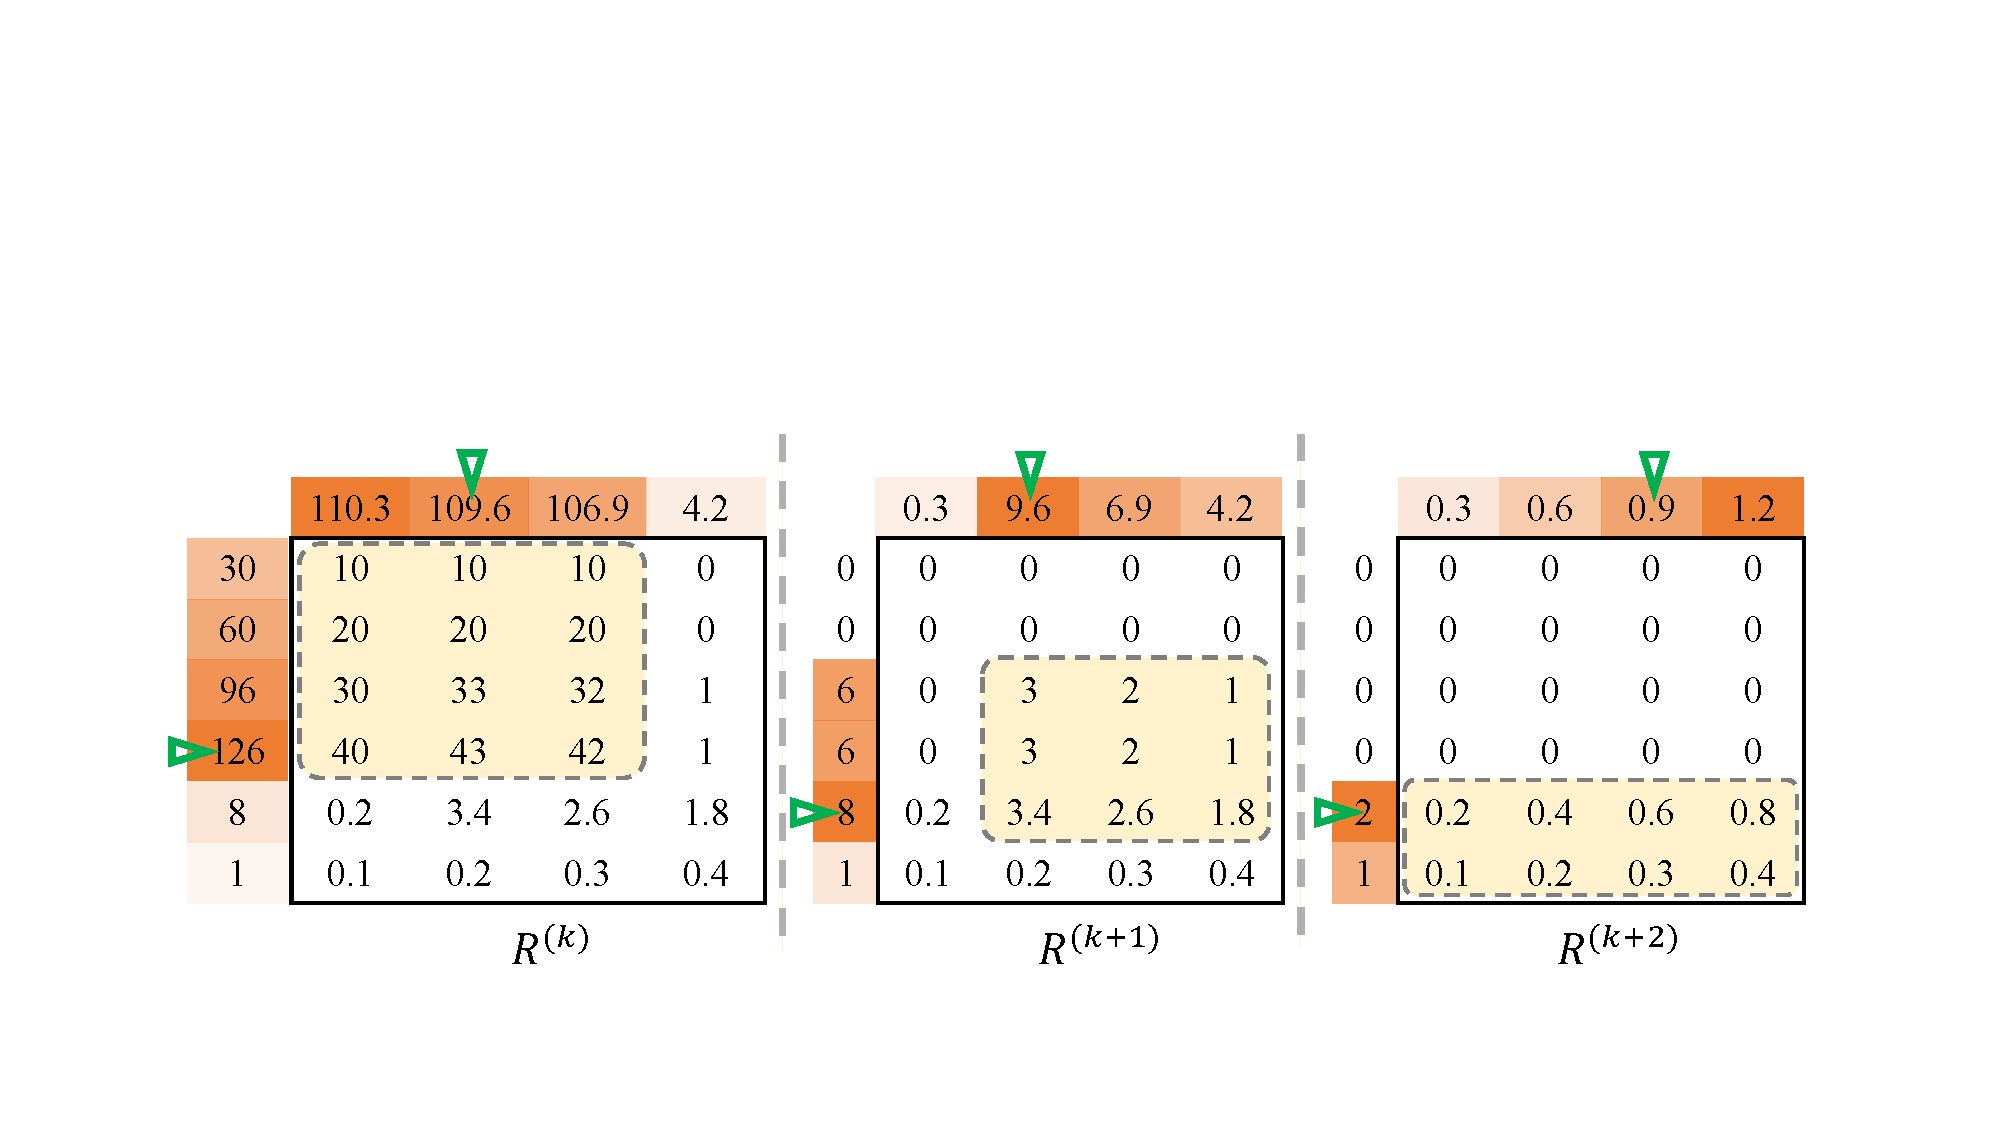
\includegraphics[width=\textwidth]{pics/MF.pdf}
\caption{评分矩阵中核心用户和核心商品的选取} \label{MF}
\end{figure}
\noindent 注意商品$i_1$和商品$i_2$之间的相似度也类似地计算,不再赘述。故,通过定义一个用户相似阈值$d_u$和商品相似阈值$d_i$,我们就能找到核心用户的邻居集$\mathcal{N}_u$和核心商品的邻居集$\mathcal{N}_i$。图\ref{MF}给了一个残差矩阵$R^{(k)}$,旁边颜色深浅代表抽样的概率大小。当绿色三角代表的核心用户与商品被抽样后,子矩阵也随之构造了出来。

\smallsection{社交网络、商品属性中的邻居选取}
在大数据时代,大量的数据可以帮助研究者们进行挖掘研究工作。例如在 LBSN中,社交网络和POI的信息可以很容易地获取到。故为了方便从POI属性中提取出一个POI网络。为了选取用户邻居$u^{(k),}$和商品邻居$i^{(k)}$,我们做两个假设:1) 用户$u$的朋友和该用户有着同样的兴趣爱好。2)用户如果访问过地点$i$,则大概率也会访问周围的地点。基于这两种假设,我们可以选取核心用户$u$和核心商品$i$的另一种邻居,分别记做:$\mathcal{F}_u$和$\mathcal{F}_i$。图\ref{BLOMA}给出了核心用户$u$与核心商品$i$的两种邻居:$\mathcal{N}_u, \mathcal{F}_u$ and $\mathcal{N}_i, \mathcal{F}_i$。



\begin{figure}[t!]
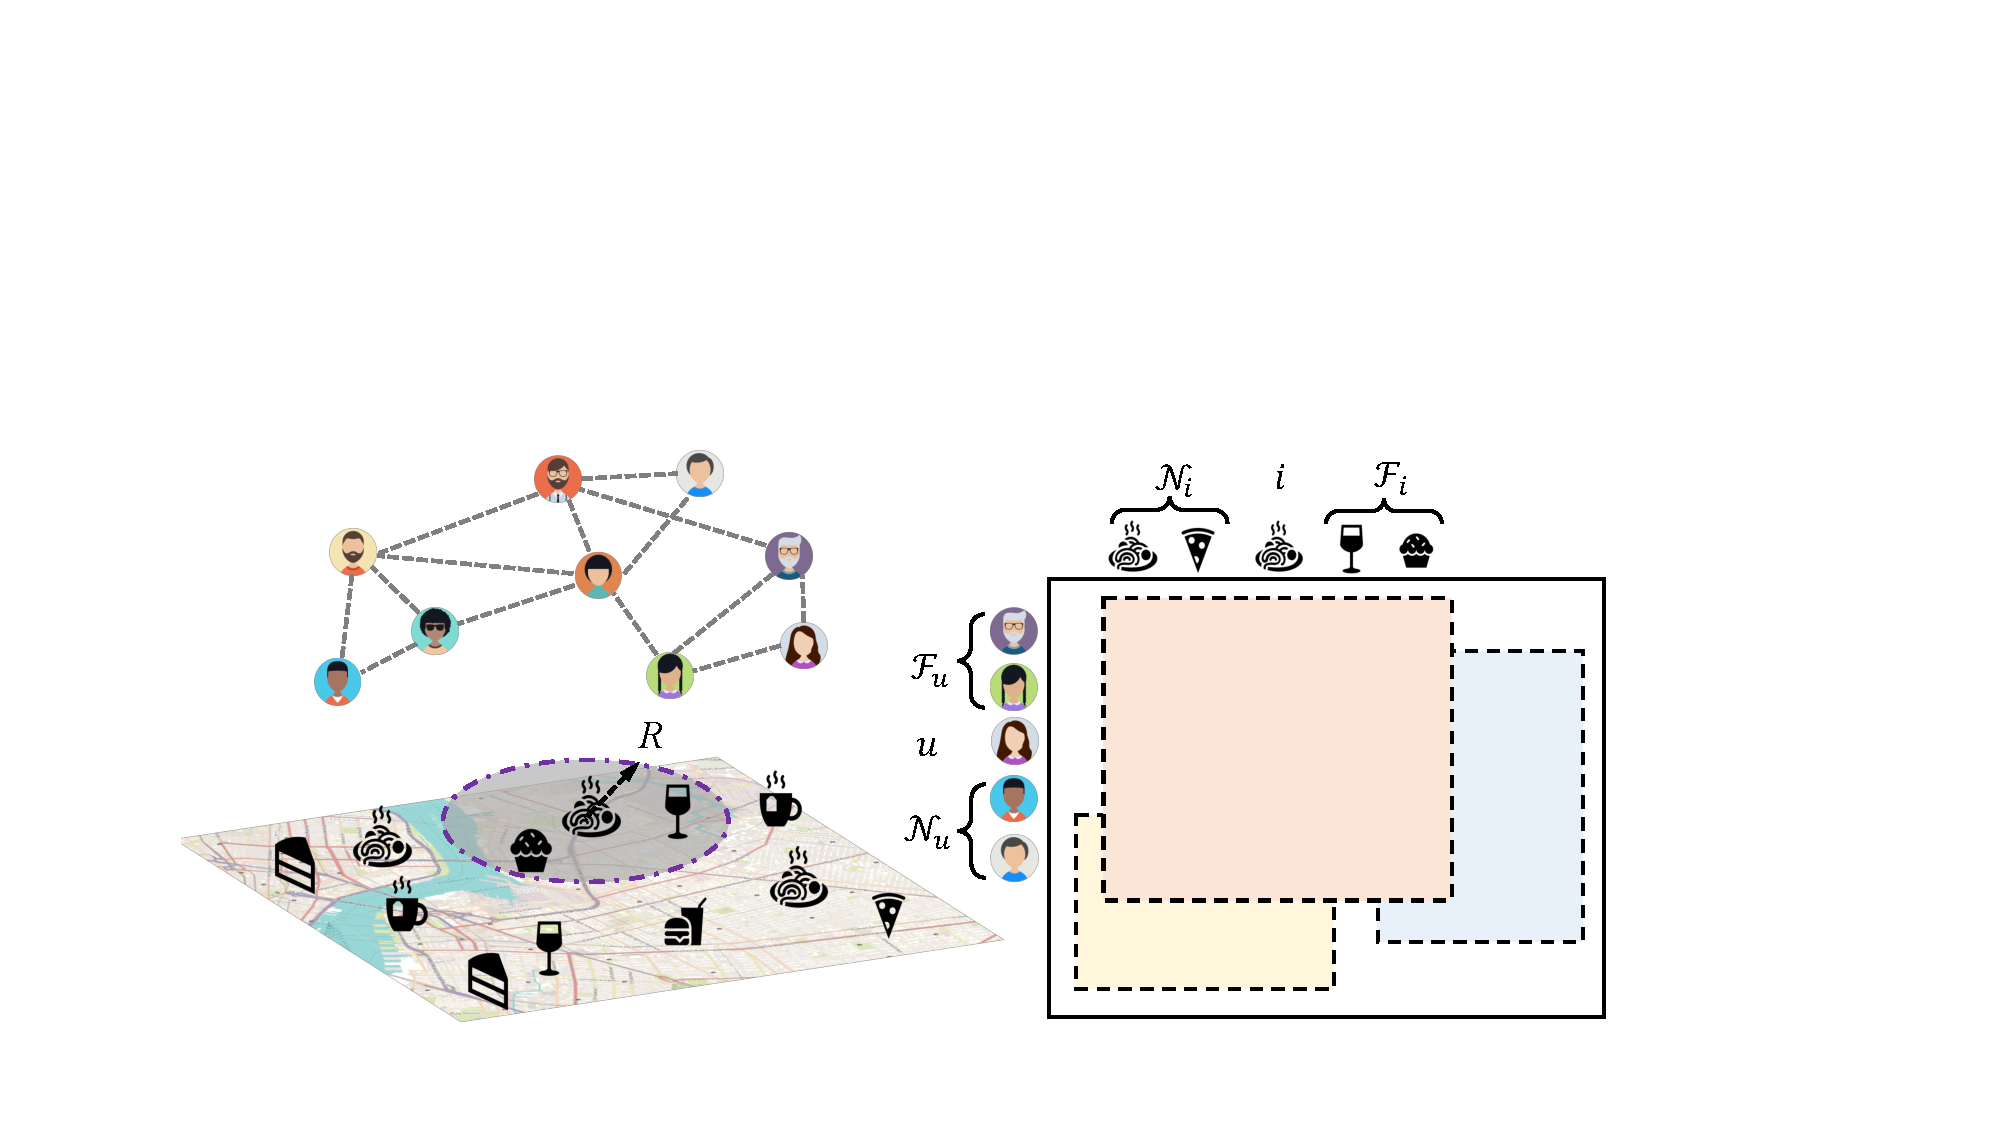
\includegraphics[width=\textwidth]{pics/BLOMA.pdf}
\caption{两种邻居的选取示意图} 
\label{BLOMA}
\end{figure}
\subsection{推荐模型}
对于每一个阶段的残差矩阵$R^{(k)}$,我们在选取核心用户、商品以及它们的邻居之后,可以用式(\ref{base})来进行分解。这里我们综合考虑多源数据,将LBSN的社交信息和地点属性也考虑了进去。这部分思想可参照工作\citeup{koren2008factorization,ma2011learning,yang2017social,guo2016novel,yin2013lcars,wang2018cross,zhang2018exploiting}。一般地,这些信息可根据约束项加进去,但在本文中,我们考虑如下的目标方程:
\begin{align}
\label{cost}
\argmin_{U^{(k)},V^{(k)}} & \Big\|\mathbb{I}\Big(R^{(k)}- g\Big(\big(\alpha U^{(k)} + (1-\alpha) SU^{(k)}\big) \cdot
\big(\beta V^{(k)} + (1-\beta)V^{(k)}T\big)\Big)\Big)\Big\|^2_F \notag\\
& + \frac{\lambda_1}{2}\|{U^{(k)}}\|_F^2 + \frac{\lambda_2}{2}\|{V^{(k)}}\|_F^2,
\end{align}
其中$U^{(k)} \in \mathbb{R}^{m\times1}$是一个表示所有用户的列向量(一维表示一个用户),$V^{(k)} \in \mathbb{R}^{1\times n}$ 是一个表示所有商品的行向量。$S\in\mathbb{R}^{m\times m}$和$T\in\mathbb{R}^{n\times n}$是用户和地点的邻接矩阵,我们将其归一化使得$\sum_u S(\cdot,u)=1$ and $\sum_i T(i,\cdot)=1$。 $\alpha$和$\beta$控制用户、商品自身和邻居所占比重的稀疏。$\mathcal{I}$是一个只是函数,如果$\mathbb{I}_{u,i} = 1$,则用户$u$曾经在地点$i$进行过交互。$g(x) = 1/(1+e^{-x})$是逻辑斯蒂函数。让不同的数据集有相同的尺度。注意评分矩阵$R$已经归一化到$(0,1)$的范围内了。

残差矩阵$R^{(k+1)}$可由集成学习的思想计算为:
\begin{equation}
\label{residue2}
R^{(k+1)} =  R^{(k)}-g\Big(\big(\alpha U^{(k)} + (1-\alpha) SU^{(k)}\big) \cdot
\big(\beta V^{(k)} + (1-\beta)V^{(k)}T\big)\Big),
\end{equation}
其中$R^{(1)} = R$是归一化后的评分矩阵。最终我们将用户向量按列连接起来得到$U = [U^{(1)}, U^{(2)}, \cdots, U^{(K)}]$,将商品向量按行连接起来得到$V = [V^{(1)}; V^{(2)}; \cdots; V^{(K)}]$。

式(\ref{cost})的求解可用交叉梯度求解法来交叉地对$U^{(k)}, V^{(k)}$进行迭代求解。最终算法的伪代码写在算法\ref{algorithm}中。

\begin{algorithm}[!t]
\caption{BLOMA算法}
\label{algorithm}
\SetKwData{True}{True}
\SetKwData{False}{False}
\SetKwFunction{Sample}{Sample}
\SetKwFunction{Count}{Count}
\SetKwFunction{Map}{Map}
\SetKwFunction{Length}{Length}
\SetKwFunction{Reduce}{Reduce}
\SetKwFunction{AverageKnn}{AverageKnn}
\SetKwFunction{RandomlyInit}{RandomlyInit}
\SetKwFunction{ROINetworkConstructor}{ROINetworkConstructor}
\SetKwFunction{Sync}{Sync}
\SetKwProg{Function}{Function}{:}{}
\SetKwInOut{Input}{Input}
\SetKwInOut{Output}{Output}
\SetKwInOut{Parameter}{Parameter}
% \small
\Input{评分矩阵$R$;用户与商品的邻接矩阵$S,T$;}
\Output{用户与商品的隐因子矩阵$U, V$;}
\BlankLine
$R^{(1)} = R; ~~k=1$;\\
\While{$\|R^{(k)}\|_F > e^{-4} $}{
$u \leftarrow$ 以$\sum_i|(R_{u,i}^{(k)})|/\sum_{u,i}|(R_{u,i}^{(k)})|$的概率抽样一个核心用户; \\
$i \leftarrow$ 以$\sum_u|(R_{u,i}^{(k)})|/\sum_{u,i}|(R_{u,i}^{(k)})|$的概率抽样一个核心商品; \\
$\mathcal{N}_u, \mathcal{N}_i \leftarrow$ 从残差矩阵中找到核心用户、商品的邻居; \\
$\mathcal{F}_u, \mathcal{F}_i \leftarrow$ 从邻接矩阵$S,T$中找到核心用户、商品的邻居; \\
$U^{(k)},V^{(k)} \leftarrow$ 用梯度下降法求解第$k$阶段的用户与商品隐因子;\\
$R^{(k+1)} \leftarrow$ 用式(\ref{residue2})计算残差矩阵;\\
k = k + 1;
}
$U = [U^{(1)}, U^{(2)}, \cdots, U^{(k)}]$; $V = [V^{(1)}; V^{(2)}; \cdots; V^{(k)}]$;\\
\end{algorithm}


\section{实验设计}
在本节中,我们将介绍实验的详细信息,包括数据集,评估指标,比较算法。并对提出模型的准确性和可解释性进行对比评价。最后给出了实验结果的分析。

\subsection{实验设置}

\smallsection{数据集}
本次试验用到了两个广为人知的推荐数据集:Filmtrust \footnote{\url{https://www.librec.net/datasets.html}}和Yelp \footnote{\url{https://www.yelp.com/dataset}}。其中Filmtrust数据只有社交信息没有商品属性,而Yelp有用户和商品的网络信息。为了方便,我们用一种简单的方法构造地点网络,即如果两个地点间的距离小于$d$的话,它们将以$p$的概率在地点网络上产生一条连边。本文我们设置$d=50$千米,$p = 0.01$。Yelp数据集中,我们移除了评分不够$100$的用户以及评分不够$200$的商品。表\ref{tab:datasets}总结了两个数据集的统计信息。

\tabcolsep=3pt
\begin{table}[!b]\renewcommand{\arraystretch}{1.3}
\caption{两个数据集的统计信息}
\center
\footnotesize
\begin{tabular}{ccccccc}
\hlinew{0.6pt} \textbf{数据集}& \textbf{用户数}& \textbf{商品数}& \textbf{评分数} & \textbf{用户边数} & \textbf{商品边数} & \textbf{包含商品标签}\\ 
\hlinew{0.6pt}
\textbf{Flimtrust}
& 1,508 & 2,071 & 35,497(1.14\%) & 1,853(0.082\%) & 0 & no\\
% \textbf{Gowalla}
% & 73,591 & 36,500 & 387,6869(0.144\%) & 716,612(0.013\%) & 314,943(0.024\%) & yes\\
\textbf{Yelp}
& 42,218 & 54,810 & 1,822,027(0.078\%) & 961,280(0.054\%) & 2,628,980(0.088\%) & yes\\
\hlinew{0.6pt}
\end{tabular}
\label{tab:datasets}
\end{table}

\smallsection{评判指标}
由于我们想要在准确性和可解释性方面来评估我们的方法,我们选择三个评估指标。其中平均绝对误差(MAE)和均方根误差(RMSE)可用于评估模型的准确性。
\begin{equation*}
\label{MAE}
\text{MAE} = \frac{1}{|\Omega_t|}\sum_{(u,i)\in\Omega_t}|R_{u,i} - \hat{R}_{u,i}|,
\end{equation*}
\begin{equation*}
\label{RMSE}
\text{RMSE} = \sqrt{\frac{1}{|\Omega_t|}\sum_{(u,i)\in\Omega_t}(R_{u,i} - \hat{R}_{u,i})^2},
\end{equation*}
其中$\Omega_t$表示了所有测试集中的用户-商品评分$(i,j)$。为了衡量模型的可解释性,我们用逐点互信息(Point-wise Mutual Information, PMI),定义如下:
\begin{equation*}
\label{PMI}
\text{PMI}(i_1, i_2) = \log\frac{p(i_1,i_2)}{p(i_1)p(i_2)},
\end{equation*}
其中$p(i_1,i_2)$是商品$i_1$和$i_2$在同一个类别下出现的概率,比如它们都是海鲜。$p(i)$ 是商品$i$在一个类别下出现的概率。具有高PMI分数的一对商品可视为语义上很相关,因此在推荐系统中同时处理它们是合理的。为了度量并计算主题的一致性,我们首先选择潜在向量$V ^ {k} $的前十大个商品,然后看它们的真实类别,来计算它们之间的平均PMI得分。


\smallsection{比较方法}
我们选取了国际主流的方法作为基准线:
\begin{itemize}
\item \textbf{RegSVD} \citeup{paterek2007improving}:是标准的SVD矩阵分解模型,模型里包含了用户与商品的二范数约束项。
\item \textbf{Standard NMF} 是基于Lee和Seung\citeup{NMF}提出的非负矩阵分解(NMF)。
\item \textbf{LLORMA} \citeup{lee2013local,zhang2017local}:一个基于局部低秩假设的矩阵分解模型,与我们的论文相同。但它没有像我们考虑的那样分步分解。

\item \textbf{SLOMA} \citeup{yang2017social}:利用用户之间的社交联系形成社交群体来找寻子矩阵的局部矩阵分解模型。

\item \textbf{RSTE} \citeup{ma2011learning}:一个概率矩阵分解模型,用于同时融合了用户$u$的兴趣和他/她亲密朋友的兴趣来对评分矩阵进行全局建模。 该模型与我们的BLOMA具有相同的分解模型,但它没有考虑局部近似。
\item \textbf{TrustSVD} \citeup{guo2016novel}:是一个建立在SVD++ \citeup{koren2008factorization}上的社交地点推荐模型,它通过进一步结合朋友对用户关于商品喜好的显式和隐性影响来建模。
\end{itemize}
我们将数据集按照$8:2$的比例分为了训练集与测试集,并把6个模型在同样的训练集与测试集上进行运行和对比。

\subsection{实验结果与分析}
\smallsection{预测准确率分析}
第一个实验是探索BLOMA的准确性。虽然BLOMA目标旨在提供可解释的推荐系统解释,但预测准确性决定了它是否可以落地。

\tabcolsep=3pt
\begin{table}[!tb]\renewcommand{\arraystretch}{1.5}
\center \caption{不同模型在两个数据集上的表现}
\small
\begin{tabular}{c|c|c|ccccccc}
\hlinew{0.7pt}
\textbf{数据集} & \textbf{ K } & \textbf{ Metrics } & \textbf{RegSVD} & \textbf{NMF} & \textbf{LLORMA} & \textbf{SLOMA}  & \textbf{RSTE} & \textbf{TrustSVD} & \textbf{BLOMA}\\
\hlinew{0.7pt}

\multirow{6}{*}{Filmtrust}
& \multirow{2}{*}{5} & MAE & 0.707 & 0.695 & 0.636 &0.630 & 0.631 &0.626 & \textbf{0.619}   \\
&  					 & RMSE& 0.914 & 0.914 & 0.857 &0.845 &  0.818 & 0.805 & \textbf{0.799}     \\
\cline{2-10}
& \multirow{2}{*}{10} & MAE & 0.707 & 0.677 & 0.643 & 0.633 & 0.640 & \textbf{0.626} & 0.647   \\
&      				  & RMSE& 0.914 & 0.897 & 0.866 & 0.847 & 0.834 & \textbf{0.805} & 0.844     \\
\cline{2-10}
& \multirow{2}{*}{20} & MAE & 0.707 & 0.667 & 0.653 &0.652 & 0.673  & \textbf{0.624} & 0.652   \\
&  					  & RMSE& 0.914 & 0.884 & 0.850 &0.869 &  0.892 & \textbf{0.803} & 0.878   \\
\hlinew{0.7pt}

\multirow{6}{*}{Yelp}
& \multirow{2}{*}{5}  & MAE & 0.806 & 0.777 & 0.733 & 0.734 & 0.739 & 0.721 & \textbf{0.713} \\
&  					  & RMSE& 1.033 & 1.001 & 0.941 & 0.945 & 0.950 & 0.926 & \textbf{0.907}\\
\cline{2-10}
& \multirow{2}{*}{10} & MAE & 0.806 & 0.771 & 0.745 & 0.740 & 0.755 & 0.721 & \textbf{0.716} \\
&  					  & RMSE& 1.033 & 0.993 & 0.957 & 0.950 & 0.972 & 0.926 & \textbf{0.910} \\
\cline{2-10}
& \multirow{2}{*}{20} & MAE & 0.806 & 0.745 & 0.760 & 0.758 & 0.827 & 0.721 & \textbf{0.720} \\
&  					  & RMSE& 1.033 & 0.957 & 0.973 & 0.972 & 1.089 & \textbf{0.926} & 0.927    \\
\hlinew{0.7pt}

\end{tabular}
\vspace{-4mm}
\label{tab:compare}
\end{table}

\begin{figure}[!thb]
\centering
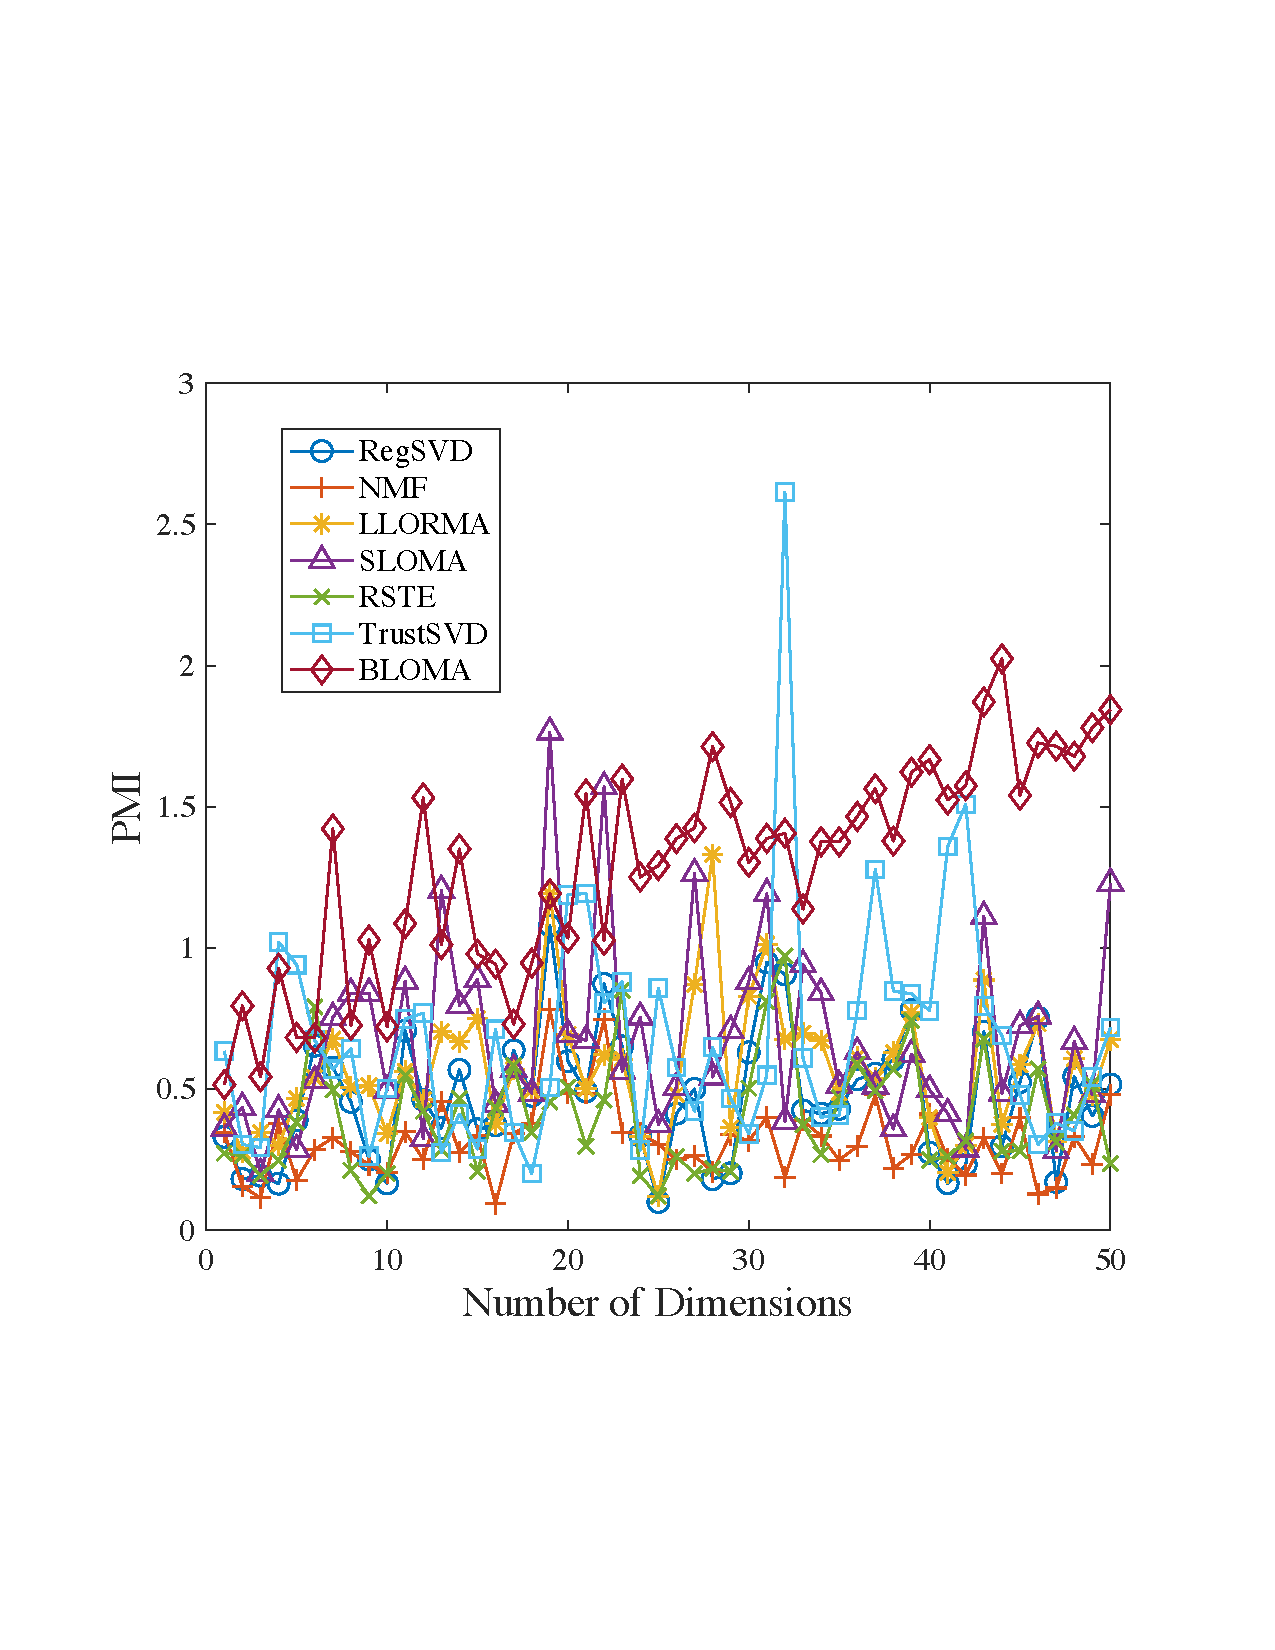
\includegraphics[width=110mm]{pics/pmi.pdf}
\caption{$50$维的地点隐矩阵的PMI指标示意图。} 
\label{pmi}
\end{figure}


表\ref{tab:compare}中可以看到BLOMA和主流方法的对比图。可以看到BLOMA打败了除了TrustSVD以外的其他算法。这一点体现出了融合多源信息的矩阵分解的高准确率。我们观察到经典的SVD和NMF模型最差的性能,原因很简单,因为他们没有考虑任何辅助信息。我们还观察到一个有趣的现象:局部MF模型(LLORMA,SLOMA,BLOMA)的性能随着$K$的增加而降低。这一点在Chen等人\citeup{chen2015wemarec}的工作中也被提到了,事实上这是算法在预测性能与可扩展性和可解释性之间的权衡,性能退化的原因是双重的。主要原因是局部模型中因子维数$K$的增加将明显地引起过度拟合。此外,局部模型不能保证子矩阵选择恰当,这将在子矩阵中引入噪声。注意TrustSVD模型的性能在所有评估中都非常好,并且随着$ K $的增加而稳定。这是因为TrustSVD是一个非常全面的模型,它考虑了评级数据中存在的所有显式和隐式信息以及社交网络中的信任信息。但其缺点是需要学习的参数太多,所以它不如其他模型那么高效。

总之,由于BLOMA已考虑合并社交和项目信息,因此可以保证预测性能。而集成学习的方式可以让矩阵分解更直观和可解释。


\begin{figure}[!t]
\centering
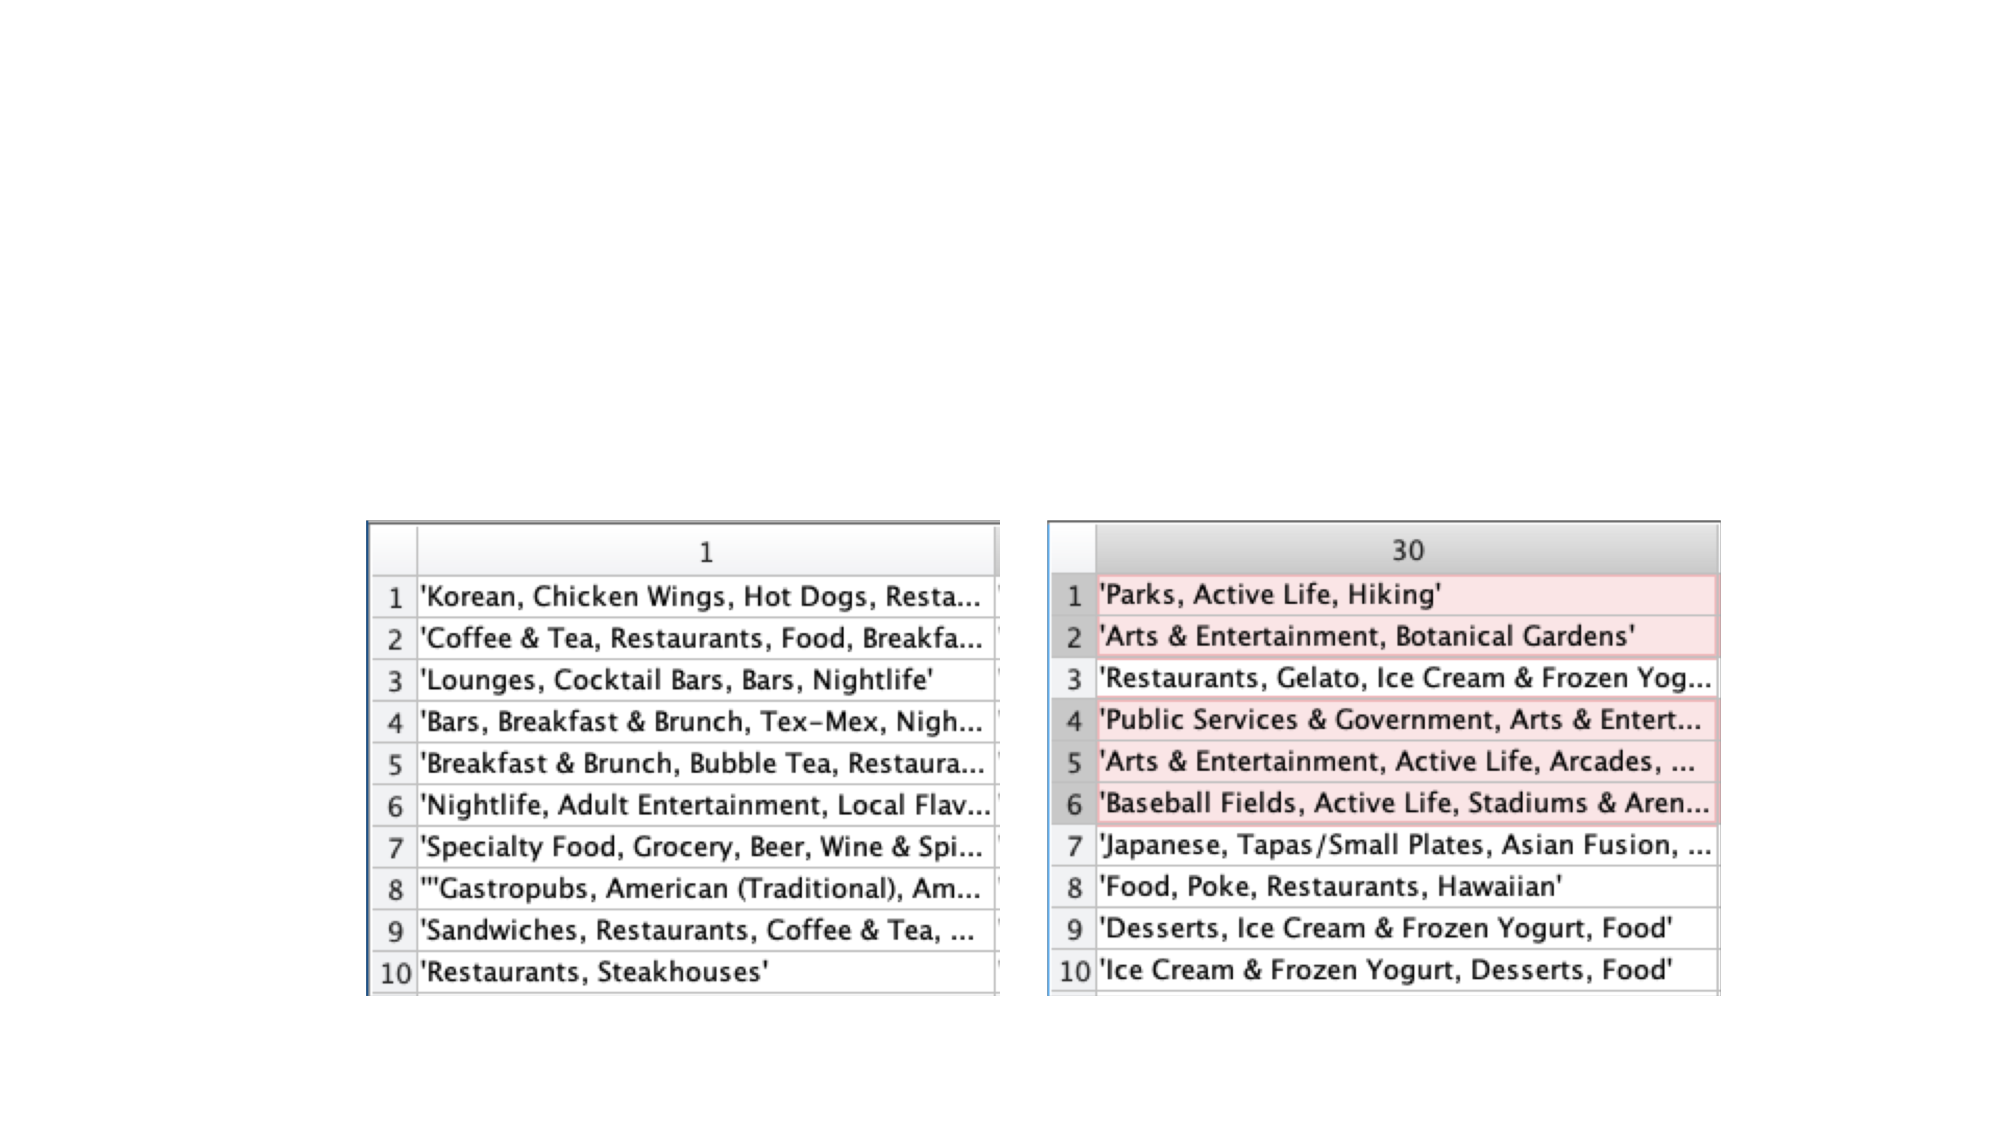
\includegraphics[width=\textwidth]{pics/factors.pdf}
\caption{在第$1$个阶段后期第$30$个阶段分解出来的地点种类可视化图。其中粉色标记了数据集中小众、不常见的类别} 
\label{factors}
\end{figure}

\smallsection{模型可解释性分析}
现在我们评估BLOMA的可解释性。正如我们在前面所述,对推荐系统的解释的目标是发现潜在隐向量中的类型信息。我们通过计算物品因子矩阵$V$上每一行具有最大绝对值的$10$个商品,并计算其两两之间的PMI。

在Yelp数据集中,有大量地点信息可供使用,但我们只需选择POI类别来计算PMI。请注意,该类别偏向于食品类和餐馆类,而其他类别比如体育类或医疗类则非常罕见。为了平衡这个问题,我们删除了拥有超过5000项的类别。

实验结果如图\ref{pmi}所示。我们可以看到BLOMA优于所有其他方法,并随着维度$ K $增加而保持着性能的优越性。这个结果反映了两个结论。首先,在开始时,通过仔细选择子索引并使用秩一分解,可以发现用户社区和具有相似语义类别的项目。其次,通过从残差矩阵(即,未解释的分量)迭代地减去局部近似分量,剩下的残差将更加清楚并且更容易解释。例如,参见图\ref{factors}。在一开始,商品集合由不同类别的东西构成,例如,食物类和酒吧类。而当BLOMA运行大约30个阶段时,地点的类别逐渐出现之前不常见到的类例如艺术类和公园类。





\section{本章小结}
\label{conclusion}
在本文中,我们提出了一种新的基于集成学习的局部矩阵分解模型。通过利用LBSN中丰富的异构信息来选择共享特征相似的用户和商品构成每次分解的子矩阵,并用秩一矩阵分解模型来进行分解。这种逐步求解的方式让矩阵分解模型更加有解释性。实验环节证明了我们的模型不仅优于最先进的算法,而且具有其他方法所没有的可解释性。
\newpage\mbox{}\thispagestyle{empty}\newpage


